
\appendix

\chapter{Notations\label{chap:Appendix-Notations}}

I chose certain notations in this book to be different from the notations
currently used in the functional programming community. The proposed
notation seems to be well adapted to reasoning about types and code,
and especially for designing data types and proving the equational
laws of typeclasses.

\section{Summary table}
\begin{description}
\item [{$F^{A}$}] type constructor $F$ with type argument $A$
\item [{$x^{:A}$}] value $x$ has type $A$
\item [{$\bbnum 1,\,1$}] the unit type and its value; in Scala, \lstinline!Unit!
and \lstinline!()!
\item [{$\bbnum 0$}] the void type; in Scala, \lstinline!Nothing!
\item [{$A+B$}] a disjunctive type; in Scala, this type is \lstinline!Either[A, B]! 
\item [{$x^{:A}+\bbnum 0^{:B}$}] a value of a disjunctive type $A+B$
\item [{$A\times B$}] a product (tuple) type; in Scala, this type is \lstinline!(A,B)!
\item [{$a^{:A}\times b^{:B}$}] value of a tuple type $A\times B$; in
Scala, \lstinline!(a, b)!
\item [{$A\Rightarrow B$}] the function type, mapping from $A$ to $B$
\item [{$x^{:A}\Rightarrow f$}] a nameless function (as a value); in Scala,
\lstinline!{ x:A => f }!
\item [{$\text{id}$}] the identity function
\item [{$\triangleq$}] ``equal by definition'' 
\item [{$\cong$}] for types, a natural isomorphism between types; for
values, ``equivalent'' values according to an established isomorphism
\item [{$A^{:F^{B}}$}] type annotation, used for defining unfunctors (GADTs) 
\item [{$\text{fmap}_{F}$}] the standard method $\text{fmap}$ pertaining
to a functor $F$ 
\item [{$\text{pu}_{F}$}] the standard method \lstinline!pure! of a monad
$F$ 
\item [{$F^{\bullet}$}] the type constructor $F$ understood as a type-level
function; in Scala, \lstinline!F[_]! 
\item [{$F^{\bullet}\leadsto G^{\bullet}$}] or $F^{A}\leadsto G^{A}$
a natural transformation between functors $F$ and $G$ 
\item [{$\forall A.P^{A}$}] a universally quantified type expression 
\item [{$\exists A.P^{A}$}] an existentially quantified type expression 
\item [{$\bef$}] the forward composition of functions: $f\bef g$ is $x\Rightarrow g(f(x))$
\item [{$\circ$}] the backward composition of functions: $f\circ g$ is
$x\Rightarrow f(g(x))$
\item [{$\circ$}] functor composition: $F\circ G$ is $F^{G^{\bullet}}$ 
\item [{$\triangleright$}] use a value as the argument of a function:
$x\triangleright f$ is $f(x)$
\item [{$f^{\uparrow G}$}] a function $f$ raised to a functor $G$; same
as $\text{fmap}_{G}f$
\item [{$f^{\uparrow G\uparrow H}$}] a function raised first to $G$ and
then to $H$; in Scala, \lstinline!h.map(_.map(f))! 
\item [{$f^{\downarrow H}$}] a function $f$ raised to a contrafunctor 
\item [{$\diamond_{M}$}] the Kleisli product operation for the monad $M$
\item [{$\oplus$}] the binary operation of a monoid; in Scala, \lstinline!x |+| y!
\item [{$\Delta$}] the ``diagonal'' function of type $\forall A.\,A\Rightarrow A\times A$
\item [{$\nabla_{1},\nabla_{2},...$}] the projections from a tuple to
its first, second, ..., parts
\item [{$\boxtimes$}] Cartesian product of functions, $(f\boxtimes g)(x)=f(x)\times g(x)$
\item [{$\left[a,b,c\right]$}] an ordered sequence of values; in Scala,
\lstinline!Seq(a, b, c)!
\item [{$\begin{array}{||cc|}
\text{id} & \bbnum 0\\
\bbnum 0 & a\Rightarrow a\times a
\end{array}$}] a function that works with disjunctive types
\end{description}

\section{Detailed explanations}

$F^{A}$ means a type constructor $F$ with a type parameter $A$.
In Scala, this is \lstinline!F[A]!. Type constructors with multiple
type parameters are denoted by $F^{A,B,C}$.

$x^{:A}$ means a value $x$ that has type $A$; this is a \textbf{\index{type annotation}type
annotation}. In Scala, a type annotation is \lstinline!x:A!. The
colon symbol, $:$, in the superscript shows that $A$ is not a type
argument (as it would be in a type constructor, $F^{A}$). The notation
$x:A$ can be used as well, but $x^{:A}$ is easier to read when $x$
is inside a larger code expression. 

$\bbnum 1$ means the unit type\index{unit type}, and $1$ means
the value of the unit type. In Scala, the unit type is \lstinline!Unit!,
and its value is denoted by \lstinline!()!. Example of using the
unit type is $\bbnum 1+A$, which in Scala corresponds to \lstinline!Option[A]!.

$\bbnum 0$ means the void\index{void type} type (the type with no
values). In Scala, this is the type \lstinline!Nothing!. Example
of using the void type is to denote the empty part of a disjunction.
For example, in the disjunction $\bbnum 1+A$ the non-empty part is
$\bbnum 0+A$, which in Scala corresponds to \lstinline!Some[A]!.
The empty part $\bbnum 1+\bbnum 0$ corresponds to \lstinline!None!.
Similarly, $A+\bbnum 0$ denotes the left part of the type $A+B$
(in Scala, \lstinline!Left[A]!), while $\bbnum 0+B$ denotes its
right part (in Scala, \lstinline!Right[A]!). Values of disjunctive
types are denoted similarly. For instance, $x^{:A}+\bbnum 0^{:B}$
denotes a value of the left part of the type $A+B$; in Scala, this
value is written as \lstinline!Left[A,B](x)!.

$A+B$ means the disjunctive type made from types $A$ and $B$ (or,
a disjunction of $A$ and $B$). In Scala, this is the type \texttt{}\lstinline!Either[A, B]!.

$x^{:A}+\bbnum 0^{:B}$ denotes a value of a disjunctive type $A+B$,
where $x$ is the value of type $A$, which is the chosen case, and
$\bbnum 0$ stands for other possible cases. For example, $x^{:A}+\bbnum 0^{B}$
is \lstinline!Left[A,B](x)! in Scala. Type annotations $^{:A}$ and
$^{:B}$ may be omitted if the types are unambiguous from the context.

$A\times B$ means the product type made from types $A$ and $B$.
In Scala, this is the tuple type \lstinline!(A,B)!.

$a^{:A}\times b^{:B}$ means a value of a tuple type $A\times B$;
in Scala, this is the tuple value \lstinline!(a, b)!. Type annotations
$^{:A}$ and $^{:B}$ may be omitted if the types are unambiguous
from the context.

$A\Rightarrow B$ means a function type from $A$ to $B$. In Scala,
this is the function type \lstinline!A => B!.

$x^{:A}\Rightarrow y$ means a nameless function with argument $x$
of type $A$ and function body $y$. (Usually, the body $y$ will
be an expression that uses $x$.) Type annotation $^{:A}$ may be
omitted if the type is unambiguous from the context.

$\text{id}$ means the identity function. The type of its argument
should be either specified as $\text{id}^{A}$ or $\text{id}^{:A\Rightarrow A}$,
or else should be unambiguous from the context. 

$\triangleq$ means ``equal by definition''. Examples:
\begin{itemize}
\item $f\triangleq(x^{:\text{Int}}\Rightarrow x+10)$ is a definition of
a function $f$. In Scala, this is written as \lstinline!val f = { x: Int => x + 10 }!
\item $F^{A}\triangleq\bbnum 1+A$ is a definition of a type constructor
$F$. In Scala, this is written as \lstinline!type F[A] = Option[A]!
\end{itemize}
$\cong$ for types means a natural isomorphism between types. For
example, $A+A\times B\cong A\times\left(\bbnum 1+B\right)$. The same
symbol $\cong$ for \emph{values} means ``equivalent'' according
to an equivalence relation that needs to be established in the text.
For example, if we have established the equivalence that allows nested
tuples to be reordered whenever needed, we can write $\left(a\times b\right)\times c\cong a\times\left(b\times c\right)$,
meaning that these values are mapped to each other by the established
isomorphism. 

$A^{:F^{B}}$ in type expressions means that the type constructor
$F^{\bullet}$ assigns the type $F^{B}$ to the type expression $A$.
This notation is used for defining unfunctors (GADTs). For example,
the Scala code

\begin{lstlisting}
sealed trait F[A]
case class F1() extends F[Int]
case class F2[A](a: A) extends F[(A, String)]
\end{lstlisting}
defines an unfunctor\index{unfunctor}, which I denote as $F^{A}\triangleq\bbnum 1^{:F^{\text{Int}}}+A^{:F^{A\times\text{String}}}$.

$\text{fmap}_{F}$ means the standard method $\text{fmap}$ of the
\lstinline!Functor! typeclass, implemented for the functor $F$.
In Scala, this may be written as \texttt{}\lstinline!Functor[F].fmap!.
Since each functor $F$ has its own specific implementation of $\text{fmap}_{F}$,
the subscript ``$F$'' is not a type parameter of $\text{fmap}_{F}$.
The method $\text{fmap}_{F}$ actually has \emph{two} type parameters,
which can be written out as $\text{fmap}_{F}^{A,B}$. Then the type
signature of $\text{fmap}$ is written in full as $\text{fmap}_{F}^{A,B}:\left(A\Rightarrow B\right)\Rightarrow F^{A}\Rightarrow F^{B}$.
For clarity, we may sometimes write explicitly the type parameters
$A,B$ in the expression $\text{fmap}_{F}^{A,B}$, but in most cases
these type parameters $A$, $B$ can be omitted without loss of clarity.
As another example, a monad's standard method \lstinline!pure! is
denoted by $\text{pu}_{F}$, where the subscript refers to the monad
$F$. This function has type signature $A\Rightarrow F^{A}$ that
contains a type parameter $A$. In the short notation, the presence
of the type parameter $A$ can be denoted by $\text{pu}_{F}^{A}$.
If we are using the \lstinline!pure! method with a complicated type,
e.g. $\bbnum 1+P^{A}$, instead of the type parameter $A$, we might
want to write this type parameter for clarity and write $\text{pu}_{F}^{\bbnum 1+P^{A}}$.
The type signature of that function is then 
\[
\text{pu}_{F}^{1+P^{A}}:\bbnum 1+P^{A}\Rightarrow F^{\bbnum 1+P^{A}}\quad.
\]
But in most cases we will not need to write the type parameter.

$F^{\bullet}$ means the type constructor $F$ understood as a type-level
function, \textendash{} that is, with a type argument unspecified.
In Scala, this is \lstinline!F[_]!. The bullet symbol, $\bullet$,
is used as a placeholder for the missing type parameter. I also simply
write $F$ when no type argument is needed, and it means the same
as $F^{\bullet}$. (For example, ``a functor $F$'' and ``a functor
$F^{\bullet}$'' mean the same thing.) However, it is useful for
clarity to be able to indicate the place where the type argument would
appear. For instance, functor composition is clearly denoted as $F^{G^{\bullet}}$;
in Scala, this is \texttt{}\lstinline!F[G[?]]! when using the ``kind
projector'' plugin.\footnote{\href{https://github.com/typelevel/kind-projector}{https://github.com/typelevel/kind-projector}}
As another example, $T_{L}^{M,\bullet}$ denotes a monad transformer
for the base monad $L$ and the foreign monad $M$. The foreign monad
$M$ is a type parameter in $T_{L}^{M,\bullet}$, and so is the missing
type parameter denoted by the placeholder symbol $\bullet$. (However,
the base monad $L$ is not a type parameter in $T_{L}^{M,\bullet}$
because the construction of the monad transformer depends sensitively
on the internal details of $L$.)

$F^{\bullet}\leadsto G^{\bullet}$ or $F^{A}\leadsto G^{A}$ means
a natural transformation between two functors $F$ and $G$. In some
Scala libraries, this is denoted by \lstinline!F ~> G!.

$\forall A.P^{A}$ is a universally quantified type expression, in
which $A$ is a bound type parameter.

$\exists A.P^{A}$ is an existentially quantified type expression,
in which $A$ is a bound type parameter.

$\bef$ means the forward composition\index{forward composition}
of functions: $f\bef g$ (reads ``$f$ before $g$'') is the function
defined as $x\Rightarrow g(f(x))$.

$\circ$ means the backward composition\index{backward composition}
of functions: $f\circ g$ (reads ``$f$ after $g$'') is the function
defined as $x\Rightarrow f(g(x))$.

$\circ$ with type constructors means their functor composition, for
example $F\circ G$ denotes the functor $F^{G^{\bullet}}$. In Scala,
this is \lstinline!F[G[A]]!. 

$x\triangleright f$ means that $x$ is inserted as the argument into
the function $f$. This \textbf{forwarding notation\index{forwarding notation}},
$x\triangleright f$, means the same expression as $f(x)$ or $f\,x$.
In Scala, the expression $x\triangleright f$ is written as \lstinline!x.f!
and is the syntax used with many standard methods such as \lstinline!.size!
or \lstinline!.toSeq!. Because the function $f$ is to the \emph{right}
of $x$ in this notation, we can chain forward compositions of functions
as $x\triangleright f\triangleright g$ in a left-associative manner,
similarly to how this is done in Scala code, for example \lstinline!x.toSeq.sorted!.
The operation $\triangleright$ binds weaker than the forward composition
$\bef$ and so $x\triangleright f\bef g=x\triangleright f\triangleright g$
in this notation. Reasoning about code in the forwarding notation
uses the identities
\begin{align*}
x\triangleright f=f(x),\quad\quad & \left(x\triangleright f\right)\triangleright g=x\triangleright f\triangleright g\quad,\\
x\triangleright f\bef g=x\triangleright\left(f\bef g\right),\quad\quad & x\triangleright f\triangleright g=x\triangleright f\bef g\quad.
\end{align*}
Some examples of reasoning in the forwarding notation:
\begin{align*}
 & \left(a\Rightarrow a\triangleright f\right)=\left(a\Rightarrow f(a)\right)=f\quad,\\
 & x\triangleright\left(y\Rightarrow a\triangleright y\right)=a\triangleright x=x(a)\quad,\\
 & x\triangleright y\triangleright f\neq x\triangleright\left(y\triangleright f\right)=f(y)(x)\quad.
\end{align*}

$f^{\uparrow G}$ means a function $f$ raised to a functor $G$.
For a function $f^{:A\Rightarrow B}$, the application of $f^{\uparrow G}$
to a value $g:G^{A}$ is written as $f^{\uparrow G}g$ or $g\triangleright f^{\uparrow G}$.
In Scala, this is \lstinline!g.map(f)!. Nested raising (i.e.~raising
to the functor composition $H\circ G$) can be written as $f^{\uparrow G\uparrow H}$,
which means $\left(f^{\uparrow G}\right)^{\uparrow H}$ and produces
a function of type $H^{G^{A}}\Rightarrow H^{G^{B}}$. Applying a nested
raising to a value $h$ of type $H^{G^{A}}$ is written as $f^{\uparrow G\uparrow H}h$
or $h\triangleright f^{\uparrow G\uparrow H}$. In Scala, this is
\lstinline!h.map(_.map(f))!. 

$f^{\downarrow H}$ means a function $f$ lifted to a contrafunctor
$H$. For a function $f^{:A\Rightarrow B}$, the application of $f^{\downarrow H}$
to a value $h:H^{B}$ is written as $f^{\downarrow H}h$ or $h\triangleright f^{\downarrow H}$,
and yields a value of type $H^{A}$. In Scala, this is \lstinline!h.contramap(f)!.

$\diamond_{M}$ means the Kleisli product operation for the monad
$M$. This is a binary operation working on two Kleisli functions
of types $A\Rightarrow M^{B}$ and $B\Rightarrow M^{C}$ and yields
a new function of type $A\Rightarrow M^{C}$.

$\oplus$ means the binary operation of a monoid, for example $x\oplus y$.
The specific monoid type should be defined for this expression to
make sense. For example, in Scala the monoidal operation is usually
denoted by \lstinline!x |+| y!.

$\Delta$ means the standard ``diagonal'' function of type $\forall A.\,A\Rightarrow A\times A$.
There is only one implementation of this type signature,
\begin{lstlisting}
def delta[A](a: A): (A, A) = (a, a)
\end{lstlisting}

$\nabla_{1},\nabla_{2},...$ denote the standard projection functions
from a tuple to its first, second, ..., parts. In Scala, $\nabla_{1}$
is \lstinline!_._1!. 

$\boxtimes$ means the component-wise Cartesian product of functions,
where the result is a pair of the values of the two functions: $(f\boxtimes g)(x)=f(x)\times g(x)$.
In Scala, this operation can be defined by
\begin{lstlisting}
def boxtimes[A,P,Q](f: A => P, g: A => Q): A => (P, Q) = x => (f(x), g(x))
\end{lstlisting}
The operations $\Delta$, $\nabla_{i}$, and $\boxtimes$ allow us
to write concisely the code for functions operating on tuples. Reasoning
about that code uses the identities
\begin{align*}
 & \Delta\bef\nabla_{i}=\text{id}\quad,\\
 & f\bef\Delta=\Delta\bef(f\boxtimes f)\quad,\\
 & (f\boxtimes g)\bef\nabla_{1}=\nabla_{1}\bef f\quad,\\
 & (f\boxtimes g)\bef\nabla_{2}=\nabla_{2}\bef g\quad.
\end{align*}

$\left[a,b,c\right]$ means an ordered sequence of values, such as
a list or an array. In Scala, this can be \lstinline!List(a, b, c)!,
\lstinline!Vector(a, b, c)!, \lstinline!Array(a, b, c)!, or another
collection type.

$f^{:Z+A\Rightarrow Z+A\times A}\triangleq\begin{array}{||cc|}
\text{id} & \bbnum 0\\
\bbnum 0 & a\Rightarrow a\times a
\end{array}$ is an example of the ``short matrix notation'' for a function that
inputs a disjunctive type and outputs another disjunctive type. In
Scala, the function $f$ is implemented as
\begin{lstlisting}
def f[Z, A]: Either[Z, A] => Either[Z, (A, A)] = {
  case Left(z)   => Left(z) // Identity function on z.
  case Right(a)  => Right((a, a)) // Delta on a.
}
\end{lstlisting}
The rows of the matrix indicate the different \lstinline!case!s in
the function's code, corresponding to the different parts of the input
disjunctive type. If the input type is not disjunctive, there will
be only one row. The columns of the matrix indicate the parts of the
output disjunctive type. If the the output type is not disjunctive,
there will be only one column.

The ``long matrix notation'' writes out all parts of the disjunctive
types in a separate ``type row'' and ``type column'':
\begin{equation}
f\triangleq\begin{array}{|c||cc|}
 & Z & A\times A\\
\hline Z & \text{id} & \bbnum 0\\
A & \bbnum 0 & a\Rightarrow a\times a
\end{array}\quad.
\end{equation}
This notation clearly indicates the input and the output types of
the function, and may be useful at the initial stages of reasoning
about the code. The vertical double line separates input types from
the function code. The ``type column'' shows the parts of the input
disjunction type $Z+A$. The ``type row'' shows the parts of the
output disjunction type $Z+A\times A$.

The matrix notation is adapted to \emph{forward} function compositions.
Assume that $A$ is a monoid type, and consider the composition of
the function $f$ shown above and the function $g$ defined by the
Scala code
\begin{lstlisting}
def g[Z, A: Monoid]: Either[Z, (A, A)] => A = {
  case Left(_)          => Monoid[A].empty
  case Right((a1, a2))  => a1 |+| a2
}
\end{lstlisting}
In the long and the short matrix notations, the function $g$ is written
as
\[
g\triangleq\begin{array}{|c||c|}
 & A\\
\hline Z & \_\Rightarrow e^{:A}\\
A\times A & a_{1}\times a_{2}\Rightarrow a_{1}\oplus a_{2}
\end{array}\quad,\quad\quad g\triangleq\begin{array}{||c|}
\_\Rightarrow e^{:A}\\
a_{1}\times a_{2}\Rightarrow a_{1}\oplus a_{2}
\end{array}\quad.
\]
The forward composition $f\bef g$ is computed by forward-composing
the matrix elements with the rules of the ordinary matrix multplication,
where any terms containing $\bbnum 0$ are omitted:
\begin{align*}
f\bef g & =\begin{array}{||cc|}
\text{id} & \bbnum 0\\
\bbnum 0 & a\Rightarrow a\times a
\end{array}\bef\begin{array}{||c|}
\_\Rightarrow e^{:A}\\
a_{1}\times a_{2}\Rightarrow a_{1}\oplus a_{2}
\end{array}\\
 & =\begin{array}{||c|}
\text{id}\bef(\_\Rightarrow e^{:A})\\
\left(a\Rightarrow a\times a\right)\bef\left(a_{1}\times a_{2}\Rightarrow a_{1}\oplus a_{2}\right)
\end{array}=\begin{array}{||c|}
\_\Rightarrow e^{:A}\\
a\Rightarrow a\oplus a
\end{array}\quad.
\end{align*}
Applying a function to a value of a disjunctive type such as $x:Z+A$
is computed by writing $x$ as a single-row matrix, for example
\[
x=z^{:Z}+\bbnum 0^{:A}=\begin{array}{||cc|}
z^{:Z} & \bbnum 0\end{array}\quad,
\]
and the computation $x\triangleright f\bef g$ again follows the rules
of matrix multiplication:
\[
x\triangleright f\bef g=\begin{array}{||cc|}
z^{:Z} & \bbnum 0\end{array}\triangleright\begin{array}{||c|}
\_\Rightarrow e^{:A}\\
a\Rightarrow a\oplus a
\end{array}=z\triangleright(\_\Rightarrow e^{:A})=e^{:A}\quad.
\]
Since the standard rules of matrix multiplication are associative,
the properties of the $\triangleright$-notation such as $x\triangleright(f\bef g)=(x\triangleright f)\triangleright g$
are guaranteed to hold.

\chapter{Glossary of terms\label{chap:Appendix-Glossary-of-terms}}

I chose certain terms in this book to be different from the terms
currently used in the functional programming community. My proposed
terminology is designed to help readers understand and remember the
concepts behind the terms. 
\begin{description}
\item [{\index{nameless�function}Nameless~function}] An expression of
function type, representing a function. For example, \lstinline!(x: Int) => x * 2!.
Also known as function expression, function literal, anonymous function,
closure, lambda-function, lambda-expression, or simply a ``lambda''.
\item [{\index{contrafunctor}Contrafunctor}] A type constructor having
the properties of a contravariant functor with respect to a type parameter.
Instead of saying ``contravariant functor'', I use the shorter name
``contrafunctor''.
\item [{\index{profunctor}Profunctor}] A type constructor whose type parameter
occurs in both covariant and contravariant positions.
\item [{\index{product�type}Product~type}] A type representing several
values given at once. In Scala, product types are the tuple types,
for example \lstinline!(Int, String)!, and case classes. Also known
as \textbf{\index{tuple type}tuple} type, \textbf{struct} (in C and
C++), and \textbf{record}.
\item [{\index{disjunctive�type}Disjunctive~type}] A type representing
one of several distinct possibilities. In Scala, this is usually implemented
as a sealed trait extended by several case classes. The standard Scala
disjunction types are \lstinline!Option[A]! and \lstinline!Either[A, B]!.
Also known as \textbf{\index{sum type}sum }type, \textbf{tagged union\index{tagged union type}}
type, \textbf{co-product\index{co-product type}} type, and variant
type (in Object Pascal and in OCaml). The shortest name is ``sum
type,'' but the English word ``sum'' is more ambiguous to the ear
than ``disjunction''.
\item [{\index{polynomial�functor}Polynomial~functor}] A type constructor
built using disjunctions (sums), products (tuples), type parameters
and fixed types. For example, in Scala, \lstinline!type F[A] = Either[(Int, A), A]!
is a polynomial functor with respect to the type parameter \lstinline!A!,
while \lstinline!Int! is a fixed type (not a type parameter). Polynomial
functors are also called \textbf{algebraic data types}\index{algebraic data type}.
A polynomial type constructor is always a functor with respect to
any of its type parameters, hence I use the shorter name ``polynomial
functor'' instead of ``polynomial type constructor''.
\item [{\index{unfunctor}Unfunctor}] A type constructor that cannot possibly
be a functor, nor a contrafunctor, nor a profunctor. An example is
a type constructor with explicitly indexed type parameters, such as
$F^{A}\triangleq\left(A\times A\right)^{:F^{\text{Int}}}+\left(\text{Int}\times A\right)^{:F^{\bbnum 1}}$.
The Scala code for this type constructor is
\begin{lstlisting}
sealed trait F[A]
final case class F1[A](x: A, y: A) extends F[Int]
final case class F2[A](s: Int, t: A) extends F[Unit]
\end{lstlisting}
Also called a \textbf{\index{GADT (generalized algebraic data type)}GADT}
(generalized algebraic data type).
\item [{\index{functor block}Functor~block}] A short syntax for composing
several \lstinline!.map!, \lstinline!.flatMap!, and \lstinline!.filter!
operations applied to a functor-typed value. The type constructor
corresponding to that value must therefore be fixed throughout the
entire functor block. (The type constructor \emph{must} be a functor
and may additionally be filterable and/or monadic.) For example, in
Scala the code
\begin{lstlisting}
for { x <- List(1,2,3); y <- List(10, x); if y > 2 }
  yield 2 * y
\end{lstlisting}
is equivalent to the code
\begin{lstlisting}
List(1, 2, 3).flatMap(x => List(10, x))
  .filter(y => y > 1).map(y => 2 * y)
\end{lstlisting}
and computes the value \lstinline!List(20, 20, 20, 6)!. This is a
functor block that ``raises'' computations to the \lstinline!List!
functor. Similar syntax exists in a number of languages and is called
a \textbf{for-comprehension\index{for-comprehension}} or list comprehension
in Python, \textbf{do-notation\index{do-notation (Haskell)}} or do-block
in Haskell, and \textbf{computation expressions\index{computation expressions (F##)@computation expressions (F\#\#)}}
in F\#. I use the name ``functor block'' in this book because it
is shorter and more descriptive. (The type constructor does not have
to)
\item [{\index{method}Method}] This word is used in two ways: 1) A method$_{1}$
is a Scala function defined as a member of a typeclass. For example,
\lstinline!flatMap! is a method defined in the \lstinline!Monad!
typeclass. 2) A method$_{2}$ is a Scala function defined as a member
of a data type declared as a Java-compatible \lstinline!class! or
\lstinline!trait!. Trait methods$_{2}$ are necessary in Scala when
implementing functions whose arguments have type parameters (because
Scala function values defined via \lstinline!val! cannot have type
parameters). So, many typeclasses such as \lstinline!Functor! or
\lstinline!Monad!, whose methods$_{1}$ require type parameters,
will use Scala \lstinline!traits! with methods$_{2}$ for their implementation.
The same applies to type constructions with quantified types, such
as the Church encoding. 
\item [{\index{Kleisli�function}Kleisli~function}] Also called a Kleisli
morphism\index{Kleisli morphism} or a \index{Kleisli arrow}Kleisli
arrow. A function with type signature $A\Rightarrow M^{B}$ for some
fixed monad $M$. More verbosely, ``a morphism from the Kleisli category
corresponding to the monad $M$''. The standard monadic method $\text{pure}_{M}:A\Rightarrow M^{A}$
has the type signature of a Kleisli function. The Kleisli product
operation, $\diamond_{M}$, is a binary operation that combines two
Kleisli functions (of types $A\Rightarrow M^{B}$ and $B\Rightarrow M^{C}$)
into a new Kleisli function (of type $A\Rightarrow M^{C}$).
\item [{\index{exponential-polynomial�type}Exponential-polynomial~type}] A
type constructor built using disjunctions (sums), products, and function
types, as well as type parameters or fixed types. For brevity, I call
them ``exp-poly'' types. For example, in Scala, \lstinline!type F[A] = Either[(A, A), Int  A]!
is an exp-poly type constructor. Such type constructors can be functors,
contrafunctors, or profunctors.
\item [{\index{short�type�notation}Short~type~notation}] A mathematical
notation for type expressions developed in this book for the purpose
of quicker and more practical reasoning about types in functional
programs. Disjunction types are denoted by $+$, product types by
$\times$, and function types by $\Rightarrow$. The unit type is
denoted by $\bbnum 1$, and the void type by $\bbnum 0$. The function
arrow $\Rightarrow$ has weaker precedence than $+$, which is in
turn weaker than $\times$. This means
\[
Z+A\Rightarrow Z+A\times A\quad\text{is the same as}\quad\left(Z+A\right)\Rightarrow\left(Z+\left(A\times A\right)\right)\quad.
\]
 Type parameters are denoted by superscripts. As an example of using
these conventions, the Scala definition\texttt{}
\begin{lstlisting}
type F[A] = Either[(A, A  Option[Int]), String  List[A]]
\end{lstlisting}
is written in the short type notation as 
\[
F^{A}\triangleq A\times\left(A\Rightarrow\bbnum 1+\text{Int}\right)+\left(\text{String}\Rightarrow\text{List}^{A}\right)\quad.
\]
\end{description}

\section{On the current misuse of the term ``algebra''}

In this book, I do not use the terms ``algebra\index{algebra}''
or ``algebraic\index{algebraic}'', because these terms are too
ambiguous. In the current practice, the functional programming community
is using the word ``algebra'' in at least \emph{four} incompatible
ways.

\paragraph{Definition 0.}

In mathematics, an \textquotedblleft algebra\textquotedblright{} is
a vector space with multiplication and certain standard properties.
For example, we need $1*x=x$, the addition must be commutative, the
multiplication must be distributive over addition, and so on. The
set of all $10\times10$ matrices with real coefficients is an \textquotedblleft algebra\textquotedblright{}
in this sense. These matrices form a $100$-dimensional vector space,
and they can be multiplied and added. This definition of ``algebra''
is not actually used in functional programming.

\paragraph{Definition 1.}

An ``algebra'' is a function with type signature $F^{A}\Rightarrow A$,
where $F^{A}$ is some fixed functor. This definition comes from category
theory, where such types are called \textbf{$F$-algebras\index{$F$-algebra}}.
There is no direct connection between this ``algebra'' and Definition~0,
except when the functor $F$ is defined by $F^{A}\triangleq A\times A$,
and then a function of type $A\times A\Rightarrow A$ may be interpreted
as a ``multiplication'' operation (but, in any case, $A$ is a type
and not a vector space, and there are no distributivity or commutativity
laws). I prefer to call such functions ``$F$-algebras'', emphasizing
that they characterize and depend on a chosen functor $F$. However,
$F$-algebras are not mentioned in this book: knowing how to reason
about their theoretical properties does not give much help in practical
programming.

\paragraph{Definition 2.}

Polynomial functors are often called \textquotedblleft algebraic data
types\textquotedblright . However, they are not \textquotedblleft algebraic\textquotedblright{}
in the sense of Definitions~0 or 1. For example, consider the \textquotedblleft algebraic
data type\textquotedblright{} \lstinline!Either[Option[A], Int]!,
which is $F^{A}\triangleq1+A+\text{Int}$ in the short type notation.
The set of all values of the type $F^{A}$ does not admit the addition
and multiplication operations required by the mathematical definition
of ``algebra''. The type $F^{A}$ may admit some binary or unary
operations (e.g.~that of a monoid), but these operations will not
be commutative or distributive. Also, there cannot be a function with
type $F^{A}\Rightarrow A$, as required for Definition~1. It seems
that the usage of the word ``algebra'' here is to refer to ``school-level
algebra'' with polynomials; these data types are built from sums
and products of types. In this book, I call such types ``polynomial''.
However, if the data type contains a function type, e.g.~\lstinline!Option[Int => A]!,
the type is no longer polynomial. So I use the more precise terms
\textquotedblleft polynomial type\textquotedblright{} and \textquotedblleft exponential-polynomial
type\textquotedblright .

\paragraph{Definition 3.}

People talk about the \textquotedblleft algebra\textquotedblright{}
of properties of functions such as \lstinline!map! or \lstinline!flatMap!,
referring to the fact that these functions must satisfy certain equational
laws (e.g.~the composition, naturality, or associativity laws). But
these laws do not form an ``algebra'' in the sense of Definition~0,
nor do the functions such as map or \lstinline!flatMap! themselves
(there are no binary operations on them). Neither do they form an
$F$-algebra in the sense of Definition~1. The laws for \texttt{}\lstinline!map!
or \lstinline!flatMap! are in no way related to \textquotedblleft algebraic
data types\textquotedblright{} of Definition~2. So here the word
\textquotedblleft algebra\textquotedblright{} is used in a way that
is unrelated to the three previous definitions. It does not actually
seem helpful to say the word ``algebra'' or ``algebraic'' when
talking about equational laws. These laws are ``algebraic'' in a
trivial sense \textendash{} they are written as equations containing
compositions of functions and applications of functions to arguments.
In mathematics, it makes sense to talk about ``algebraic'' equations
as different from ``differential'' or ``integral'' equations.
In functional programming, all equational laws are of the same kind:
some code on the left-hand side must be equal to some code on the
right-hand side of the equation. Since functional programming does
not have ``non-algebraic'' laws, calling its laws ``algebraic''
does not clarify anything. I call them ``equational laws'' or just
``laws'' in this book.

\paragraph{Definition 4.}

In the Church encoding of a free monad (nowadays known as the ``final
tagless'' encoding), the term ``algebra'' refers to the function
$S^{E^{\bullet}}\leadsto E^{\bullet}$, which is a sub-expression
of the Church encoding $\forall E^{\bullet}.\,(S^{E^{\bullet}}\leadsto E^{\bullet})\Rightarrow E^{A}$
that uses the \emph{type constructor} parameter $E$. This definition
is related only to Definition~1 if we consider $S^{E}\leadsto E$
as an $S$-algebra in the category of \emph{functors}. The fact that
$S^{E^{\bullet}}\leadsto E^{\bullet}$ is an $S$-algebra in the category
of functors does not provide any additional insight or help for practical
work with the Church encoding of a free monad.

In some online tutorials, the type constructor $S$ itself is called
an ``algebra''. The type constructor $S$ is used to parameterize
the effects described by the Church-encoded free monad, so I call
it the ``effect constructor''.

So, it seems that the current usage of the word ``algebra'' in functional
programming is both inconsistent and unhelpful to practitioners. In
this book, I reserve the word ``algebra'' to denote the branch of
mathematics, as in ``school-level algebra'' or ``graduate-level
algebra''. Instead of ``algebra'' as in Definitions~1 to 4, I
talk about ``$F$-algebras'' with a specific functor $F$; ``polynomial
types'' or ``polynomial functors'' or ``exponential-polynomial
functors'' etc.; ``equational laws''; and an ``effect constructor''
$S$.

\chapter{Scala syntax and features}

\subsection{Function syntax}

Functions have arguments, body, and type. The function type lists
the type of all arguments and the type of the result value.
\begin{lstlisting}
def f(x: Int, y: Int): Int => Int = { z => x + y + z }
\end{lstlisting}

Functions may be used with \index{infix syntax}infix syntax as well.
For this syntax to work, the function must be defined \textbf{as a
Scala method}\index{method}\index{Scala method}, that is, using
\texttt{def} within the declaration of \texttt{x}'s class, or as an
extension method. The infix syntax cannot work with functions defined
using \texttt{val}. For clarity, I call Scala functions \textbf{infix
methods}\index{infix method} when defined and used in this way.

The syntax \texttt{}\lstinline!List[Int]! means ``a list of integer
values.'' In the type expression \lstinline!List[Int]!, the ``\texttt{}\lstinline!Int!''
is called the \textbf{type parameter\index{type parameter}} and \texttt{}\lstinline!List!
is called the \textbf{type constructor}\index{type constructor}. 

A list can contain values of any type; for example, \texttt{}\lstinline!List[List[List[Int]]]!
means a list of lists of lists of integers. So, a type constructor
can be seen as a function from types to types. A type constructor
takes a type parameter as an argument, and produces a new type as
a result.

\subsection{Functions of several arguments vs.~tuples}

In Scala, there is a difference between a function whose argument
is a tuple,
\begin{lstlisting}
def f1(p: (Int, String)): Int = ???
\end{lstlisting}
and a function with several arguments,
\begin{lstlisting}
def f2(x: Int, s: String): Int = ???
\end{lstlisting}
This difference is ``cosmetic'' because these functions are equivalent
from the computational point of view. However, Scala syntax for these
functions is different.

\subsection{Scala collections}

The Scala standard library defines collections of several kinds, the
main ones being sequences, sets, and dictionaries. These collections
have many map/reduce-style methods defined on them.

Sequences are ``subclasses'' of the class \texttt{Seq}. The standard
library will sometimes choose automatically a suitable subclass of
\texttt{Seq}, such as \texttt{List}, \texttt{IndexedSeq}, \texttt{Vector},
\texttt{Range}, etc.; for example:
\begin{lyxcode}
scala>~1~to~5

scala>~(1~to~5).map(x~=>~x{*}x)

scala>~(1~to~5).toList

scala>~1~until~5

scala>~(1~until~5).toList
\end{lyxcode}
For our purposes, all these ``sequence-like'' types are equivalent.

Sets are values of class \texttt{Set}, and dictionaries are values
of class \texttt{Map}.
\begin{lyxcode}
scala>~Set(1,~2,~3).filter(x~$\Rightarrow$~x~\%~2~==~0)
\end{lyxcode}

\chapter{The Curry-Howard correspondence\label{app:The-Curry-Howard-correspondence}}

\section{Slides}

Type constructions in functional programming

The common ground between OCaml, Haskell, Scala, Rust, and other languages

Type constructions common in FP languages:

Tuple (``product'') type: $\text{Int}\times\text{String}$

Function type: $\text{Int}\Rightarrow\text{String}$

Disjunction (``sum'') type: $\text{Int}+\text{String}$

Unit type (``empty tuple''): $1$

Type parameters: $\text{List}^{T}$

Up to differences in syntax, the FP languages share all these features

Type constructions: Scala syntax

Tuple type: \texttt{\textcolor{blue}{\footnotesize{}(Int, String)}}{\footnotesize\par}

Create: \texttt{\textcolor{blue}{\footnotesize{}val pair:\ (Int,
String) = (123, \textquotedbl abc\textquotedbl )}} 

Use: \texttt{\textcolor{blue}{\footnotesize{}val y:\ String = pair.\_2}}{\footnotesize\par}

Function type: \texttt{\textcolor{blue}{\footnotesize{}Int $\Rightarrow$
String}}{\footnotesize\par}

Create: \texttt{\textcolor{blue}{\footnotesize{}def f:\ (Int $\Rightarrow$
String) = x $\Rightarrow$ \textquotedbl Value is \textquotedbl{}
+ x.toString}} 

Use: \texttt{\textcolor{blue}{\footnotesize{}val y:\ String = f(123)}}{\footnotesize\par}

Disjunction type: \texttt{\textcolor{blue}{\footnotesize{}Either{[}Int,
String{]}}} defined in standard library

Create:\\
 \texttt{\textcolor{blue}{\footnotesize{}\ val x:\ Either{[}Int,
String{]} = Left(123)}}~\\
\texttt{\textcolor{blue}{\footnotesize{} val y:\ Either{[}Int, String{]}
= Right(\textquotedbl abc\textquotedbl )}}{\footnotesize\par}

Use: \texttt{\textcolor{blue}{\footnotesize{}val z:\ Boolean = x
match \{}}~\\
\texttt{\textcolor{blue}{\footnotesize{} case Left(i) $\Rightarrow$
i > 0}}~\\
\texttt{\textcolor{blue}{\footnotesize{} case Right(\_) $\Rightarrow$
false}}~\\
\texttt{\textcolor{blue}{\footnotesize{}\}}}{\footnotesize\par}

Unit type: \texttt{\textcolor{blue}{\footnotesize{}Unit}}{\footnotesize\par}

Create: \texttt{\textcolor{blue}{\footnotesize{}val x:\ Unit = ()}}{\footnotesize\par}

Type constructions: OCaml syntax

Tuple type: \texttt{\textcolor{blue}{\footnotesize{}int {*} string}}{\footnotesize\par}

Create: \texttt{\textcolor{blue}{\footnotesize{}let pair:\ int {*}
string = (123, \textquotedbl abc\textquotedbl )}} 

Use: \texttt{\textcolor{blue}{\footnotesize{}let y:\ string = snd
pair}}{\footnotesize\par}

Function type: \texttt{\textcolor{blue}{\footnotesize{}int -> string}}{\footnotesize\par}

Create: \texttt{\textcolor{blue}{\footnotesize{}let f:\ int -> string
=}}~\\
\texttt{\textcolor{blue}{\footnotesize{} fun x -> Printf.sprintf \textquotedbl Value
is \%d\textquotedbl{} x}} 

Use: \texttt{\textcolor{blue}{\footnotesize{}let y:\ string = f 123}}{\footnotesize\par}

Disjunction type: \texttt{\textcolor{blue}{\footnotesize{}type e =
Left of int | Right of string}}{\footnotesize\par}

Create:\\
 \texttt{\textcolor{blue}{\footnotesize{}\ let x:\ e = Left 123}}~\\
\texttt{\textcolor{blue}{\footnotesize{} let y:\ e = Right \textquotedbl abc\textquotedbl}}{\footnotesize\par}

Use: \texttt{\textcolor{blue}{\footnotesize{}let z:\ bool = match
x with}}~\\
\texttt{\textcolor{blue}{\footnotesize{} Left i -> i > 0}}~\\
\texttt{\textcolor{blue}{\footnotesize{} Right \_ -> false}}~\\

Unit type: \texttt{\textcolor{blue}{\footnotesize{}unit}}{\footnotesize\par}

Create: \texttt{\textcolor{blue}{\footnotesize{}let x:\ unit = ()}}{\footnotesize\par}

Type constructions: Haskell syntax

Tuple type: \texttt{\textcolor{blue}{\footnotesize{}(Int, String)}}{\footnotesize\par}

Create: \texttt{\textcolor{blue}{\footnotesize{}pair = (123, \textquotedbl abc\textquotedbl )}} 

Use: \texttt{\textcolor{blue}{\footnotesize{}(\_, y) = pair}}{\footnotesize\par}

Function type: \texttt{\textcolor{blue}{\footnotesize{}Int -> String}}{\footnotesize\par}

Create: \texttt{\textcolor{blue}{\footnotesize{}f = \textbackslash x
-> \textquotedbl Value is \textquotedbl{} ++ show x}} 

Use: \texttt{\textcolor{blue}{\footnotesize{}y = f 123}}{\footnotesize\par}

Disjunction type: \texttt{\textcolor{blue}{\footnotesize{}data E =
Left Int | Right String}}{\footnotesize\par}

Create:\\
\  \texttt{\textcolor{blue}{\footnotesize{}x = Left 123}}~\\
\texttt{\textcolor{blue}{\footnotesize{} y = Right \textquotedbl abc\textquotedbl}}{\footnotesize\par}

Use: \texttt{\textcolor{blue}{\footnotesize{}z = case x of}}~\\
\texttt{\textcolor{blue}{\footnotesize{} Left i -> i > 0}}~\\
\texttt{\textcolor{blue}{\footnotesize{} Right \_ -> false}}~\\

Unit type: \texttt{\textcolor{blue}{\footnotesize{}Unit}}{\footnotesize\par}

Create: \texttt{\textcolor{blue}{\footnotesize{}x = ()}}{\footnotesize\par}

From types to propositions

The code \texttt{\textcolor{blue}{\footnotesize{}val x:\ T =}} ...
shows that \emph{we can compute a value} of type \texttt{\textcolor{blue}{\footnotesize{}T}}
as part of our program expression

Let's denote this \emph{proposition} by ${\cal CH}(T)$ \textendash{}
``$\mathcal{C}$ode $\mathcal{H}$as a value of type \texttt{\textcolor{blue}{\footnotesize{}T}}''

Correspondence between types and propositions, for a given program:
\begin{center}
\begin{tabular}{|c|c|c|}
\hline 
\textbf{Type} & \textbf{Proposition} & \textbf{Short notation}\tabularnewline
\hline 
\hline 
\texttt{\textcolor{blue}{\footnotesize{}T}} & ${\cal CH}(T)$ & $T$\tabularnewline
\hline 
\texttt{\textcolor{blue}{\footnotesize{}(A, B)}} & ${\cal CH}(A)$ \emph{and} ${\cal CH}(B)$ & $A\wedge B$; $A\times B$\tabularnewline
\hline 
\texttt{\textcolor{blue}{\footnotesize{}Either{[}A, B{]}}} & ${\cal CH}(A)$ \emph{or} ${\cal CH}(B)$ & $A\vee B$; $A+B$\tabularnewline
\hline 
\texttt{\textcolor{blue}{\footnotesize{}A $\Rightarrow$ B}} & ${\cal CH}(A)$ \emph{implies} ${\cal CH}(B)$ & $A\Rightarrow B$\tabularnewline
\hline 
\texttt{\textcolor{blue}{\footnotesize{}Unit}} & \emph{True} & 1\tabularnewline
\hline 
\end{tabular}
\par\end{center}

Type parameter \texttt{\textcolor{blue}{\footnotesize{}{[}T{]}}} in
a function type means $\forall T$

Example: \texttt{\textcolor{blue}{\footnotesize{}def dupl{[}A{]}:\ A
$\Rightarrow$ (A, A)}}. The type of this function, $A\Rightarrow A\times A$,
corresponds to the theorem $\forall A:A\Rightarrow A\wedge A$

Translating language constructions into the logic I

How to represent logical relationships between ${\cal CH}(...)$ propositions?

Code expressions create\,\emph{logical relationships} between propositions
${\cal CH}(...)$

``Logical relationships'' = what will be true if something given
is true

The elementary proof task is represented by a \textbf{sequent}

Notation: $A,B,C\vdash G$; the \textbf{premises} are $A,B,C$ and
the \textbf{goal} is G

Proofs are achieved via axioms and derivation rules

Axioms: such and such sequents are already true

Derivation rules: this sequent is true if such and such sequents are
true

To make connection with logic, represent code fragments as \textbf{sequents}

\textcolor{blue}{$A,B\vdash C$} represents an \emph{expression} of
type \texttt{\textcolor{blue}{\footnotesize{}C}} that uses \texttt{\textcolor{blue}{\footnotesize{}x:\ A}}
and \texttt{\textcolor{blue}{\footnotesize{}y:\ B}}{\footnotesize\par}

Examples in Scala:

\texttt{\textcolor{blue}{\footnotesize{}(x:\ Int).toString + \textquotedbl abc\textquotedbl}}
is an expression of type \texttt{\textcolor{blue}{\footnotesize{}String}}
that uses an \texttt{\textcolor{blue}{\footnotesize{}x:\ Int}} and
is represented by the sequent $\text{Int}\vdash\text{String}$

\texttt{\textcolor{blue}{\footnotesize{}(x:\ Int) $\Rightarrow$
x.toString + \textquotedbl abc\textquotedbl}} is an expression
of type \texttt{\textcolor{blue}{\footnotesize{}Int $\Rightarrow$
String}} and is represented by the sequent $\emptyset\vdash\text{Int}\Rightarrow\text{String}$

Sequents only describe the \emph{types} of expressions and their parts

Translating language constructions into the logic II

What are the derivation rules for the logic of types?

Write all the constructions in FP languages as sequents

This will give all the derivation rules for the logic of types

Each type construction has an expression for creating it and an expression
for using it

Tuple type $A\times B$

Create: $A,B\vdash A\times B$ 

Use: $A\times B\vdash A$ and also $A\times B\vdash B$

Function type $A\Rightarrow B$

Create: if we have $A\vdash B$ then we will have $\emptyset\vdash A\Rightarrow B$ 

Use: $A\Rightarrow B,A\vdash B$

Disjunction type $A+B$

Create: $A\vdash A+B$ and also $B\vdash A+B$

Use: $A+B,A\Rightarrow C,B\Rightarrow C\vdash C$

Unit type $1$

Create: $\emptyset\vdash1$

Translating language constructions into the logic III

Additional rules for the logic of types

In addition to constructions that use types, we have ``trivial''
constructions:

a single, unmodified value of type $A$ is a valid expression of type
$A$

For any $A$ we have the sequent $A\vdash A$

if a value can be computed using some given data, it can also be computed
if given\,\emph{additional} data

If we have $A,...,C\vdash G$ then also $A,...,C,D\vdash G$ for any
$D$

For brevity, we denote by $\Gamma$ a sequence of arbitrary premises

the order in which data is given does not matter, we can still compute
all the same things given the same premises in different order

If we have $\Gamma,A,B\vdash G$ then we also have $\Gamma,B,A\vdash G$

Syntax conventions:

the implication operation associates \emph{to the right}

$A\Rightarrow B\Rightarrow C$ means $A\Rightarrow\left(B\Rightarrow C\right)$

precedence order: implication, disjunction, conjunction

$A+B\times C\Rightarrow D$ means $\left(A+\left(B\times C\right)\right)\Rightarrow D$

Quantifiers: implicitly, all our type variables are universally quantified

When we write $A\Rightarrow B\Rightarrow A$, we mean $\forall A:\forall B:A\Rightarrow B\Rightarrow A$

The logic of types I

Now we have all the axioms and the derivation rules of the logic of
types.

What theorems can we derive in this logic?

Example: $A\Rightarrow B\Rightarrow A$

Start with an axiom $A\vdash A$; add an unused extra premise $B$:
$A,B\vdash A$

Use the ``create function'' rule with $B$ and $A$, get $A\vdash B\Rightarrow A$

Use the ``create function'' rule with $A$ and $B\Rightarrow A$,
get the final sequent $\emptyset\vdash A\Rightarrow B\Rightarrow A$
showing that $A\Rightarrow B\Rightarrow A$ is a \textbf{theorem}
since it is derived from no premises

What code does this describe?

The axiom $A\vdash A$ represents the expression $x^{A}$ where $x$
is of type $A$

The unused premise $B$ corresponds to unused variable $y^{B}$ of
type $B$

The ``create function'' rule gives the function $y^{B}\Rightarrow x^{A}$

The second ``create function'' rule gives $x^{A}\Rightarrow\left(y^{B}\Rightarrow x\right)$

Scala code: \texttt{\textcolor{blue}{\footnotesize{}def f{[}A, B{]}:\ A
$\Rightarrow$ B $\Rightarrow$ A = (x:\ A) $\Rightarrow$ (y:\ B)
$\Rightarrow$ x}}{\footnotesize\par}

Any code expression's type can be translated into a sequent

A proof of a theorem directly guides us in writing code for that type

Correspondence between programs and proofs

By construction, any theorem can be implemented in code
\begin{center}
\begin{tabular}{|c|c|}
\hline 
\textbf{Proposition} & \textbf{Code}\tabularnewline
\hline 
\hline 
$\forall A:A\Rightarrow A$ & \texttt{\textcolor{blue}{\footnotesize{}def identity{[}A{]}(x:\ A):\ A
= x}}\tabularnewline
\hline 
$\forall A:A\Rightarrow1$ & \texttt{\textcolor{blue}{\footnotesize{}def toUnit{[}A{]}(x:\ A): Unit
= ()}}\tabularnewline
\hline 
$\forall A\forall B:A\Rightarrow A+B$ & \texttt{\textcolor{blue}{\footnotesize{}def inLeft{[}A,B{]}(x:A):\ Either{[}A,B{]}
= Left(x)}}\tabularnewline
\hline 
$\forall A\forall B:A\times B\Rightarrow A$ & \texttt{\textcolor{blue}{\footnotesize{}def first{[}A,B{]}(p:\ (A,B)):\ A
= p.\_1}}\tabularnewline
\hline 
$\forall A\forall B:A\Rightarrow B\Rightarrow A$ & \texttt{\textcolor{blue}{\footnotesize{}def const{[}A,B{]}(x:\ A):\ B$\Rightarrow$A
= (y:B)$\Rightarrow$x}}\tabularnewline
\hline 
\end{tabular}
\par\end{center}

Also, non-theorems \emph{cannot be implemented} in code 

Examples of non-theorems:\\
 $\forall A:1\Rightarrow A$; \  \  $\quad\forall A\forall B:A+B\Rightarrow A$;
\\
$\forall A\forall B:A\Rightarrow A\times B$; \  $\quad\forall A\forall B:(A\Rightarrow B)\Rightarrow A$

Given a type's formula, can we implement it in code? Not obvious.

Example: $\forall A\forall B:((((A\Rightarrow B)\Rightarrow A)\Rightarrow A)\Rightarrow B)\Rightarrow B$

Can we write a function with this type? Can we prove this formula?

The logic of types II

What kind of logic is this? What do mathematicians call this logic?

This is called ``intuitionistic propositional logic'', IPL (also
``constructive'')

This is a ``nonclassical'' logic because it is different from Boolean
logic

Disjunction works very differently from Boolean logic

Example: $A\Rightarrow B+C\vdash(A\Rightarrow B)+(A\Rightarrow C)$
does not hold in IPL

This is counter-intuitive!

We cannot implement a function with this type:

\texttt{\textcolor{blue}{\footnotesize{}def q{[}A,B,C{]}(f: A $\Rightarrow$
Either{[}B, C{]}): Either{[}A $\Rightarrow$ B, A $\Rightarrow$ C{]}}}{\footnotesize\par}

Disjunction is ``constructive'': need to supply one of the parts

But \texttt{\textcolor{blue}{\footnotesize{}Either{[}A $\Rightarrow$
B, A $\Rightarrow$ C{]}}} is not a function of \texttt{\textcolor{blue}{\footnotesize{}A}} 

Implication works somewhat differently

Example: $\left(\left(A\Rightarrow B\right)\Rightarrow A\right)\Rightarrow A$
holds in Boolean logic but not in IPL

Cannot compute an \texttt{\textcolor{blue}{\footnotesize{}x:\ A}}
because of insufficient data

Conjunction works the same as in Boolean logic

Example: 
\[
A\Rightarrow B\times C\vdash\left(A\Rightarrow B\right)\times\left(A\Rightarrow C\right)
\]
 

The logic of types III

How to determine whether a given IPL formula is a theorem?

The IPL cannot have a truth table with a fixed number of truth values

This was shown by G\"odel in 1932 (see \href{https://en.wikipedia.org/wiki/Many-valued_logic}{Wikipedia page})

The IPL has a decision procedure (algorithm) that either finds a proof
for a given IPL formula, or determines that there is no proof

There may be several inequivalent proofs of an IPL theorem

Each proof can be \emph{automatically translated} into code

The \href{https://github.com/Chymyst/curryhoward}{curryhoward} library
implements an IPL prover as a Scala macro, and generates Scala code
from types

The \href{https://hackage.haskell.org/package/djinn-ghc}{djinn-ghc}
compiler plugin and the \href{https://github.com/nomeata/ghc-justdoit}{JustDoIt plugin}
implement an IPL prover in Haskell, and generate Haskell code from
types

All these IPL provers use the same basic algorithm called LJT 

and all cite the same paper {\footnotesize{}\href{https://rd.host.cs.st-andrews.ac.uk/publications/jsl57.pdf}{[Dyckhoff 1992]}}{\footnotesize\par}

because most other papers on this subject are incomprehensible to
non-specialists, or describe algorithms that are too complicated

Proof search I: looking for an algorithm

Why our initial presentation of IPL does not give a proof search algorithm

The FP type constructions give nine axioms and three derivation rules:

\begin{minipage}[t]{0.49\columnwidth}%
\begin{itemize}
\item $\Gamma,A,B\vdash A\times B$ 
\item $\Gamma,A\times B\vdash A$ 
\item $\Gamma,A\times B\vdash B$
\item $\Gamma,A\Rightarrow B,A\vdash B$
\item $\Gamma,A\vdash A+B$ 
\item $\Gamma,B\vdash A+B$
\item $\Gamma,A+B,A\Rightarrow C,B\Rightarrow C\vdash C$
\item $\Gamma\vdash1$
\item $\Gamma,A\vdash A$
\end{itemize}
%
\end{minipage}%
\begin{minipage}[t]{0.49\columnwidth}%
\[
\frac{\Gamma,A\vdash B}{\Gamma\vdash A\Rightarrow B}
\]
\[
\frac{\Gamma\vdash G}{\Gamma,D\vdash G}
\]
\[
\frac{\Gamma,A,B\vdash G}{\Gamma,B,A\vdash G}
\]
%
\end{minipage}

\medskip{}
Can we use these rules to obtain a finite and complete search tree?
No.

Try proving $A,B+C\vdash A\times B+C$: cannot find matching rules

Need a better formulation of the logic

Proof search II: Gentzen's calculus LJ (1935)

A ``complete and sound calculus'' is a set of axioms and derivation
rules that will yield all (and only!) theorems of the logic
\begin{align*}
\text{(}X\text{ is atomic)\,}\frac{}{\Gamma,{\color{blue}X}\vdash X}\:Id & \qquad\frac{}{\Gamma\vdash{\color{blue}\top}}\,\top\\
\frac{\Gamma,A\Rightarrow B\vdash A\quad\;\Gamma,B\vdash C}{\Gamma,{\color{blue}A\Rightarrow B}\vdash C}\:L\Rightarrow & \qquad\frac{\Gamma,A\vdash B}{\Gamma\vdash{\color{blue}A\Rightarrow B}}\,R\Rightarrow\\
\frac{\Gamma,A\vdash C\quad\;\Gamma,B\vdash C}{\Gamma,{\color{blue}A+B}\vdash C}\:L+ & \qquad\frac{\Gamma\vdash A_{i}}{\Gamma\vdash{\color{blue}A_{1}+A_{2}}}\,R+_{i}\\
\frac{\Gamma,A_{i}\vdash C}{\Gamma,{\color{blue}A_{1}\times A_{2}}\vdash C}\:L\times_{i} & \qquad\frac{\Gamma\vdash A\quad\;\Gamma\vdash B}{\Gamma\vdash{\color{blue}A\times B}}\,R\times
\end{align*}

Two axioms and eight derivation rules

Each derivation rule says: The sequent at bottom will be proved if
proofs are given for sequent(s) at top

Use these rules ``bottom-up'' to perform a proof search

Sequents are nodes and proofs are edges in the proof search tree

Proof search example I

Example: to prove $\left(\left(R\Rightarrow R\right)\Rightarrow Q\right)\Rightarrow Q$

Root sequent $S_{0}:\emptyset\vdash\left(\left(R\Rightarrow R\right)\Rightarrow Q\right)\Rightarrow Q$

$S_{0}$ with rule $R\Rightarrow$ yields $S_{1}:\left(R\Rightarrow R\right)\Rightarrow Q\vdash Q$

$S_{1}$ with rule $L\Rightarrow$ yields $S_{2}:\left(R\Rightarrow R\right)\Rightarrow Q\vdash R\Rightarrow R$
and $S_{3}:Q\vdash Q$

Sequent $S_{3}$ follows from the $Id$ axiom; it remains to prove
$S_{2}$

$S_{2}$ with rule $L\Rightarrow$ yields $S_{4}:\left(R\Rightarrow R\right)\Rightarrow Q\vdash R\Rightarrow R$
and $S_{5}:Q\vdash R\Rightarrow R$

We are stuck here because $S_{4}=S_{2}$ (we are in a loop)

We can prove $S_{5}$, but that will not help

So we backtrack (erase $S_{4}$, $S_{5}$) and apply another rule
to $S_{2}$

$S_{2}$ with rule $R\Rightarrow$ yields $S_{6}:\left(R\Rightarrow R\right)\Rightarrow Q;R\vdash R$

Sequent $S_{6}$ follows from the $Id$ axiom

Therefore we have proved $S_{0}$

Since $\left(\left(R\Rightarrow R\right)\Rightarrow Q\right)\Rightarrow Q$
is derived from no premises, it is a theorem

$Q.E.D.$

Proof search III: The calculus LJT

Vorobieff-Hudelmaier-Dyckhoff, 1950-1990

The Gentzen calculus LJ will loop if rule $L\Rightarrow$ is applied
$\geq2$ times

The calculus LJT keeps all rules of LJ except rule $L\Rightarrow$

Replace rule $L\Rightarrow$ by pattern-matching on $A$ in the premise
$A\Rightarrow B$:
\begin{align*}
\text{(}X\text{ is atomic)\,}\frac{\Gamma,X,B\vdash D}{\Gamma,X,{\color{blue}X\Rightarrow B}\vdash D}\:L\Rightarrow_{1}\\
\frac{\Gamma,A\Rightarrow B\Rightarrow C\vdash D}{\Gamma,{\color{blue}(A\times B)\Rightarrow C}\vdash D}\:L\Rightarrow_{2}\\
\frac{\Gamma,A\Rightarrow C,B\Rightarrow C\vdash D}{\Gamma,{\color{blue}(A+B)\Rightarrow C}\vdash D}\:L\Rightarrow_{3}\\
\frac{\Gamma,B\Rightarrow C\vdash A\Rightarrow B\quad\quad\Gamma,C\vdash D}{\Gamma,{\color{blue}(A\Rightarrow B)\Rightarrow C}\vdash D}\:L\Rightarrow_{4}
\end{align*}

When using LJT rules, the proof tree has no loops and terminates

See \href{http://citeseer.ist.psu.edu/viewdoc/summary\%3Fdoi\%3D10.1.1.35.2618}{this paper}
for an explicit decreasing measure on the proof tree

Proof search IV: The calculus LJT

``\emph{It is obvious that it is obvious}'' \textendash{} a mathematician
after thinking for a half-hour

Rule $L\Rightarrow_{4}$ is based on the key theorem: {\footnotesize{}
\[
\left(\left(A\Rightarrow B\right)\Rightarrow C\right)\Rightarrow\left(A\Rightarrow B\right)\,\Longleftrightarrow\,\left(B\Rightarrow C\right)\Rightarrow\left(A\Rightarrow B\right)
\]
}{\footnotesize\par}

The key theorem for rule $L\Rightarrow_{4}$ is attributed to Vorobieff
(1958):
\begin{center}
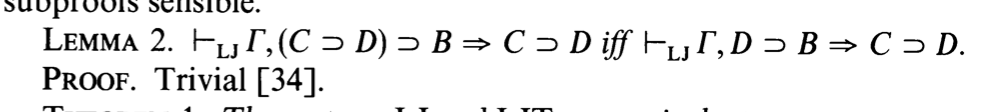
\includegraphics[width=0.8\textwidth]{Vorobieff-lemma}
\par\end{center}

\begin{center}
{\footnotesize{}{[}R. Dyckhoff, }\emph{\footnotesize{}Contraction-Free
Sequent Calculi for Intuitionistic Logic}{\footnotesize{}, 1992{]}}{\footnotesize\par}
\par\end{center}

A stepping stone to this theorem:{\footnotesize{}
\[
\left(\left(A\Rightarrow B\right)\Rightarrow C\right)\Rightarrow B\Rightarrow C
\]
}Proof (\emph{obviously} trivial): $f^{\left(A\Rightarrow B\right)\Rightarrow C}\Rightarrow b^{B}\Rightarrow f\:(x^{A}\Rightarrow b)$

\emph{Details are left as exercise for the reader}

Proof search V: From deduction rules to code

The new rules are equivalent to the old rules, therefore...

Proof of a sequent $A,B,C\vdash G$ $\Leftrightarrow$ code/expression
$t(a,b,c):G$

Also can be seen as a function $t$ from $A,B,C$ to $G$

Sequent in a proof follows from an axiom or from a transforming rule

The two axioms are fixed expressions, $x^{A}\Rightarrow x$ and $1$

Each rule has a \emph{proof transformer} function: $\text{PT}_{R\Rightarrow}$
, $\text{PT}_{L+}$ , etc.

Examples of proof transformer functions:
\begin{align*}
\frac{\Gamma,A\vdash C\quad\;\Gamma,B\vdash C}{\Gamma,{\color{blue}A+B}\vdash C}\:L+\\
PT_{L+}(t_{1}^{A\Rightarrow C},t_{2}^{B\Rightarrow C})=x^{A+B}\Rightarrow & \ x\ \text{match}\begin{cases}
a^{A}\Rightarrow t_{1}(a)\\
b^{B}\Rightarrow t_{2}(b)
\end{cases}
\end{align*}
\begin{align*}
\frac{\Gamma,A\Rightarrow B\Rightarrow C\vdash D}{\Gamma,{\color{blue}(A\times B)\Rightarrow C}\vdash D}\:L\Rightarrow_{2}\\
PT_{L\Rightarrow_{2}}(f^{\left(A\Rightarrow B\Rightarrow C\right)\Rightarrow D})=g^{A\times B\Rightarrow C}\Rightarrow & f\,(x^{A}\Rightarrow y^{B}\Rightarrow g(x,y))
\end{align*}

Verify that we can indeed produce PTs for every rule of LJT

Proof search example II: deriving code

Once a proof tree is found, start from leaves and apply PTs

For each sequent $S_{i}$, this will derive a \textbf{proof expression}
$t_{i}$

Example: to prove $S_{0}$, start from $S_{6}$ backwards:{\footnotesize{}
\begin{align*}
S_{6}:\left(R\Rightarrow R\right)\Rightarrow Q;R\vdash R\quad(\text{axiom }Id)\quad & t_{6}(rrq,r)=r\\
S_{2}:\left(R\Rightarrow R\right)\Rightarrow Q\vdash\left(R\Rightarrow R\right)\quad\text{PT}_{R\Rightarrow}(t_{6})\quad & t_{2}(rrq)=\left(r\Rightarrow t_{6}(rrq,r)\right)\\
S_{3}:Q\vdash Q\quad(\text{axiom }Id)\quad & t_{3}(q)=q\\
S_{1}:\left(R\Rightarrow R\right)\Rightarrow Q\vdash Q\quad\text{PT}_{L\Rightarrow}(t_{2},t_{3})\quad & t_{1}(rrq)=t_{3}(rrq(t_{2}(rrq)))\\
S_{0}:\emptyset\vdash\left(\left(R\Rightarrow R\right)\Rightarrow Q\right)\Rightarrow Q\quad\text{PT}_{R\Rightarrow}(t_{1})\quad & t_{0}=\left(rrq\Rightarrow t_{1}(rrq)\right)
\end{align*}
}{\footnotesize\par}

The proof expression for $S_{0}$ is then obtained as
\begin{align*}
t_{0} & =rrq\Rightarrow t_{3}\left(rrq\left(t_{2}\left(rrq\right)\right)\right)=rrq\Rightarrow rrq(r\Rightarrow t_{6}\left(rrq,r\right)\\
 & =rrq\Rightarrow rrq\left(r\Rightarrow r\right)
\end{align*}
Simplified final code having the required type: 
\[
t_{0}:\left(\left(R\Rightarrow R\right)\Rightarrow Q\right)\Rightarrow Q=\left(rrq\Rightarrow rrq\left(r\Rightarrow r\right)\right)
\]


\section{Intuitionistic propositional logic (IPL)}

The intuitionistic propositional logic (sometimes also called the
``constructive'' propositional logic) describes how programs in
functional programming languages may be able to compute values of
different types.

The main formal difference between IPL and the classical (Boolean)
logic is that IPL does not include the axiom of excluded middle (``\emph{tertium
non datur}''), which is 
\[
\forall A:(A\text{\emph{ or}}\left(\text{\emph{not}}\left(A\right)\right))\text{ is true}\quad.
\]
However, given just this information, it is not easy to understand
the consequences of \emph{not having} this axiom, or to figure out
which statements are true in the IPL. 

The reason this axiom is not included in IPL is that IPL propositions
such as ${\cal CH}(A)$ correspond to the \emph{practical possibility}
of values of type $A$ \emph{to be computed} by a program. For the
proposition ${\cal CH}(A)$ to be true in IPL, a program needs to
actually compute a value of type $A$. It is not sufficient merely
to show that the non-existence of such a value would be somehow contradictory.
But in classical logic, the axiom of excluded middle says that either
${\cal CH}(A)$ or $\text{\emph{not}}\left({\cal CH}(A)\right)$ is
true. So showing that ``$\text{\emph{not}}\left({\cal CH}(A)\right)$''
is contradictory is sufficient for proving ${\cal CH}(A)$, without
ever computing any values of type $A$. For this reason, classical
(Boolean) logic does not adequately describe the logic of types in
functional programming, i.e.~it does not correctly predict the types
of values that can be computed by functional programs.

\section{Example: The logic of types is not Boolean}

Here is an explicit example of obtaining an incorrect result when
using classical logic to reason about values computed by functional
programs. Consider the formula
\begin{equation}
\left(A\Rightarrow B+C\right)\Rightarrow\left(A\Rightarrow B\right)+\left(A\Rightarrow C\right)\label{eq:abc-example-classical-logic}
\end{equation}
or, putting in all the parentheses for clarity,
\[
\left(A\Rightarrow\left(B+C\right)\right)\Rightarrow\left(\left(A\Rightarrow B\right)+\left(A\Rightarrow C\right)\right)\quad.
\]
This formula is a true theorem in classical logic. To prove this,
we only need to show that Eq.~(\ref{eq:abc-example-classical-logic})
is always equal to \emph{true} (i.e.~Boolean value $1$) for any
Boolean values of the variables $A$, $B$, $C$. Consider that the
only way an implication $A\Rightarrow B$ could be \emph{false} (that
is, equal to $0$) in Boolean logic is when $A=1$ and $B=0$. So,
Eq.~(\ref{eq:abc-example-classical-logic}) can be false only if
$\left(A\Rightarrow B+C\right)=1$ and $\left(A\Rightarrow B\right)+\left(A\Rightarrow C\right)=0$.
The disjunction can be false only when both parts are false; so we
must have $\left(A\Rightarrow B\right)=0$ and $\left(A\Rightarrow C\right)=0$.
This is only possible if $A=1$ and $B=C=0$. But, with these value
assignments, we find $\left(A\Rightarrow B+C\right)=0$ rather than
$1$. So, we cannot ever make Eq.~(\ref{eq:abc-example-classical-logic})
equal to $0$ as a Boolean formula. This shows Eq.~(\ref{eq:abc-example-classical-logic})
to be a ``classically valid'' formula, i.e.~a theorem that holds
in classical Boolean logic.

If we use the Curry-Howard correspondence and apply Eq.~(\ref{eq:abc-example-classical-logic})
to propositions such as ${\cal CH}\left(A\right)$, ${\cal CH}\left(B\right)$,
${\cal CH}\left(C\right)$, we obtain the statement that a program
should be able to compute a value of type $\left(A\Rightarrow B\right)+\left(A\Rightarrow C\right)$
given a value of type $A\Rightarrow B+C$. In Scala, such a program
would be written as a function with the following type signature,
\begin{lstlisting}
def bad[A, B, C](g: A => Either[B, C]): Either[A=>B, A=>C] = ???
\end{lstlisting}
However, it is impossible to implement this function in Scala as a
total function.

To help build an intuition for the impossibility of implementing \lstinline!bad!,
consider that the only available data is a function $g:A\Rightarrow B+C$,
which may return values of type $B$ or $C$ depending on the input
value of type $A$. The function \lstinline!bad! must return either
a function of type $A\Rightarrow B$ or a function of type $A\Rightarrow C$.
Can we create a function of type $A\Rightarrow B$? Given a value
of type $A$, we need to compute a value of type $B$. Since the type
$B$ is completely arbitrary (it is a type parameter), we cannot produce
a value of type $B$ from scratch. The only potential source of values
of type $B$ is the input function $g$. However, $g$ may produce
values of type $C$ for some values of type $A$. So, in general,
we cannot build a function of type $A\Rightarrow B$ out of the function
$g$. Similarly, we find that we cannot build a function of type $A\Rightarrow C$
out of $g$. 

The decision about whether to return $A\Rightarrow B$ or $A\Rightarrow C$
must be somehow made in the code of \lstinline!bad!. The only input
data is the function $g$ that takes an argument of type $A$. We
could imagine calling $g$ on various arguments of type $A$ and to
see whether $g$ returns a $B$ or a $C$. However, the type $A$
is unknown, so the function \lstinline!bad! cannot produce any values
of that type and call $g$. So the decision about whether to return
$A\Rightarrow B$ or $A\Rightarrow C$ must be made regardless of
the function $g$. Whichever we choose to return, $A\Rightarrow B$
or $A\Rightarrow C$, we will not be able to return a result value
of the required type.

We could try to switch between $A\Rightarrow B$ and $A\Rightarrow C$
depending on a given value of type $A$. This, however, corresponds
to a different type signature: 
\[
\left(A\Rightarrow B+C\right)\Rightarrow A\Rightarrow\left(A\Rightarrow B\right)+\left(A\Rightarrow C\right)\quad.
\]
This type signature \emph{can} be implemented, for instance, by this
Scala code:
\begin{lstlisting}
def q[A, B, C](g: A => Either[B, C]): A => Either[A=>B, A=>C] = { a =>
  g(a) match {
    case Left(b) => Left(_ => b)
    case Right(c) => Right(_ => c)
  }
}
\end{lstlisting}
But this is not the type signature that describes Eq.~(\ref{eq:abc-example-classical-logic})
via the Curry-Howard correspondence.

In the IPL, it turns out that Eq.~(\ref{eq:abc-example-classical-logic})
is not a valid theorem, i.e.~it is impossible to find a proof of
Eq.~(\ref{eq:abc-example-classical-logic}) using the axioms and
the derivation rules of the IPL. To \emph{prove} that there is no
proof, one needs to use methods of proof theory that are beyond the
scope of this book. A good introduction to the required technique
is the book ``\emph{Proof and Disproof in Formal Logic}'' by R.~Bornat.\footnote{~\href{https://www.amazon.com/Proof-Disproof-Formal-Logic-Introduction/dp/0198530277}{R. Bornat, "Proof and Disproof in Formal Logic", Oxford, 2005 - link to Amazon.com}} 

This example illustrates that it is precisely the valid theorems in
the IPL, and not the valid theorems in the Boolean logic, that correspond
to implementable functional programs.

\section{Using truth values in Boolean logic and in IPL}

Another significant difference between IPL and the Boolean logic is
that propositions in IPL cannot be assigned a fixed set of ``truth
values''. This was proved by G�del in 1935. It means that a proposition
in IPL cannot be decided by writing out a truth table, even if we
allow more than two truth values.

\chapter{Category theory}

Examples of categories
\begin{enumerate}
\item Objects: types $\text{Int}$, $\text{String}$, ...; morphisms (arrows)
are functions $\text{Int}\rightarrow\text{String}$ etc. \textendash{}
this is the ``standard'' category corresponding to a given programming
language
\item Objects: types $A$, $B$, ...; morphisms are pairs of functions $\left(A\rightarrow B\right),\left(B\rightarrow A\right)$
\item {*} Objects: types $\text{List}^{A}$, $\text{List}^{B}$, ...; morphisms
are functions of type $\text{List}^{A}\rightarrow\text{List}^{B}$
\item Objects: types $A$, $B$, ...; morphisms are functions of type $\text{List}^{A}\rightarrow\text{List}^{B}$
\item Objects: types $A$, $B$, ...; morphisms are functions of type $A\rightarrow\text{List}^{B}$
\item {*} Objects: types $\text{List}^{A}$, $\text{List}^{B}$, ...; morphisms
are functions $A\rightarrow B$
\item Objects: types $A$, $B$, ...; morphisms are $\text{List}^{A\rightarrow B}$
\item Objects: types $A,$ $B$, ...; morphisms are functions $B\rightarrow A$
\item {*} Objects: things $A,$ $B$, ...; morphisms are pairs $\left(A,B\right)$
of things \textendash{} this is the same as a preorder
\end{enumerate}
Examples marked with {*} are for illustration only, they are probably
not very useful

\chapter{A humorous disclaimer}

\emph{The following text is quoted in part from an anonymous source
(``Project Guten Tag'') dating back at least to 1997. The original
text is no longer available on the Internet.}

\medskip{}

\noun{Warranto Limitensis; Disclamatantus Damagensis}

Solus exceptus ``Rectum Replacator Refundiens'' describitus ecci,
\begin{enumerate}
\item Projectus (etque nunquam partum quis hic etext remitibus cum \noun{Project
Guten Tag}-tm identificator) disclamabat omni liabilitus tuus damagensis,
pecuniensisque, includibantus pecunia legalitus, et 
\item \noun{Remedia Negligentitia Non Habet Tuus, Warrantus Destructi\-bus
Contractus Nullibus Ni Liabilitus Sumus, Inclutatibus Non Limitatus
Destructio Directibus, Consequentius, Punitio, O Incidentus, Non Sunt
Si Nos Notificat Vobis}. 
\end{enumerate}
Sit discubriatus defectus en etextum sic entram diariam noventam recibidio,
pecuniam tuum refundatorium receptorus posset, sic scribatis vendor.
Sit veniabat medium physicalis, vobis idem reternat et replacator
possit copius. Sit venitabat electronicabilis, sic viri datus chansus
segundibus. 

\noun{Hic Etext Venid ``Como-asi''. Nihil Warranti Nunquam Classum,
Expressito Ni Implicato, Le Macchen Como Si Etexto Bene Sit O Il Medio
Bene Sit, Inclutat Et Non Limitat Warranti Mercatensis, Appropriatensis
Purposem. }

Statuen varias non permitatent disclamabaris ni warranti implicatoren
ni exclusioni limitatio damagaren consequentialis, ecco lo qua disclamatori
exclusato\-rique non vobis applicant, et potat optia alia legali.

\chapter{GNU Free Documentation License\label{sec:GFDL} }

{\tiny{}Version 1.2, November 2002}{\tiny\par}

{\tiny{}Copyright (c) 2000,2001,2002 Free Software Foundation, Inc.
59 Temple Place, Suite 330, Boston, MA 02111-1307, USA}{\tiny\par}

{\tiny{}Everyone is permitted to copy and distribute verbatim copies
of this license document, but changing it is not allowed.}{\tiny\par}

{\tiny{}\setcounter{subsection}{-1}}{\tiny\par}

\subsection*{{\tiny{}Preamble}}

{\tiny{}The purpose of this License is to make a manual, textbook,
or other functional and useful document free in the sense of freedom:
to assure everyone the effective freedom to copy and redistribute
it, with or without modifying it, either commercially or noncommercially.
Secondarily, this License preserves for the author and publisher a
way to get credit for their work, while not being considered responsible
for modifications made by others.}{\tiny\par}

{\tiny{}This License is a kind of \textquotedblleft copyleft'', which
means that derivative works of the document must themselves be free
in the same sense. It complements the GNU General Public License,
which is a copyleft license designed for free software.}{\tiny\par}

{\tiny{}We have designed this License in order to use it for manuals
for free software, because free software needs free documentation:
a free program should come with manuals providing the same freedoms
that the software does. But this License is not limited to software
manuals; it can be used for any textual work, regardless of subject
matter or whether it is published as a printed book. We recommend
this License principally for works whose purpose is instruction or
reference.}{\tiny\par}

\subsection{Applicability and definitions\label{subsec:1Applicability-and-definitions}}

{\tiny{}This License applies to any manual or other work, in any medium,
that contains a notice placed by the copyright holder saying it can
be distributed under the terms of this License. Such a notice grants
a world-wide, royalty-free license, unlimited in duration, to use
that work under the conditions stated herein. The \textquotedblleft Document'',
below, refers to any such manual or work. Any member of the public
is a licensee, and is addressed as \textquotedblleft you''. You accept
the license if you copy, modify or distribute the work in a way requiring
permission under copyright law.}{\tiny\par}

{\tiny{}A \textquotedblleft Modified Version'' of the Document means
any work containing the Document or a portion of it, either copied
verbatim, or with modifications and/or translated into another language.}{\tiny\par}

{\tiny{}A \textquotedblleft Secondary Section'' is a named appendix
or a front-matter section of the Document that deals exclusively with
the relationship of the publishers or authors of the Document to the
Document's overall subject (or to related matters) and contains nothing
that could fall directly within that overall subject. (Thus, if the
Document is in part a textbook of mathematics, a Secondary Section
may not explain any mathematics.) The relationship could be a matter
of historical connection with the subject or with related matters,
or of legal, commercial, philosophical, ethical or political position
regarding them.}{\tiny\par}

{\tiny{}The \textquotedblleft Invariant Sections'' are certain Secondary
Sections whose titles are designated, as being those of Invariant
Sections, in the notice that says that the Document is released under
this License. If a section does not fit the above definition of Secondary
then it is not allowed to be designated as Invariant. The Document
may contain zero Invariant Sections. If the Document does not identify
any Invariant Sections then there are none.}{\tiny\par}

{\tiny{}The \textquotedblleft Cover Texts'' are certain short passages
of text that are listed, as Front-Cover Texts or Back-Cover Texts,
in the notice that says that the Document is released under this License.
A Front-Cover Text may be at most 5 words, and a Back-Cover Text may
be at most 25 words.}{\tiny\par}

{\tiny{}A \textquotedblleft Transparent'' copy of the Document means
a machine-readable copy, represented in a format whose specification
is available to the general public, that is suitable for revising
the document straightforwardly with generic text editors or (for images
composed of pixels) generic paint programs or (for drawings) some
widely available drawing editor, and that is suitable for input to
text formatters or for automatic translation to a variety of formats
suitable for input to text formatters. A copy made in an otherwise
Transparent file format whose markup, or absence of markup, has been
arranged to thwart or discourage subsequent modification by readers
is not Transparent. An image format is not Transparent if used for
any substantial amount of text. A copy that is not \textquotedblleft Transparent''
is called \textquotedblleft Opaque''.}{\tiny\par}

{\tiny{}Examples of suitable formats for Transparent copies include
plain ASCII without markup, Texinfo input format, \LaTeX{} input format,
SGML or XML using a publicly available DTD, and standard-conforming
simple HTML, PostScript or PDF designed for human modification. Examples
of transparent image formats include PNG, XCF and JPG. Opaque formats
include proprietary formats that can be read and edited only by proprietary
word processors, SGML or XML for which the DTD and/or processing tools
are not generally available, and the machine-generated HTML, PostScript
or PDF produced by some word processors for output purposes only.}{\tiny\par}

{\tiny{}The ``Title Page'' means, for a printed book, the title
page itself, plus such following pages as are needed to hold, legibly,
the material this License requires to appear in the title page. For
works in formats which do not have any title page as such, \textquotedblleft Title
Page\textquotedblright{} means the text near the most prominent appearance
of the work's title, preceding the beginning of the body of the text.}{\tiny\par}

{\tiny{}A section ``Entitled XYZ'' means a named subunit of the
Document whose title either is precisely XYZ or contains XYZ in parentheses
following text that translates XYZ in another language. (Here XYZ
stands for a specific section name mentioned below, such as \textquotedblleft Acknowledgements\textquotedblright ,
\textquotedblleft Dedications\textquotedblright , \textquotedblleft Endorsements\textquotedblright ,
or \textquotedblleft History\textquotedblright .) To \textquotedblleft Preserve
the Title\textquotedblright{} of such a section when you modify the
Document means that it remains a section \textquotedblleft Entitled
XYZ\textquotedblright{} according to this definition.}{\tiny\par}

{\tiny{}The Document may include Warranty Disclaimers next to the
notice which states that this License applies to the Document. These
Warranty Disclaimers are considered to be included by reference in
this License, but only as regards disclaiming warranties: any other
implication that these Warranty Disclaimers may have is void and has
no effect on the meaning of this License.}{\tiny\par}

\subsection{Verbatim copying\label{subsec:2Verbatim-copying}}

{\tiny{}You may copy and distribute the Document in any medium, either
commercially or noncommercially, provided that this License, the copyright
notices, and the license notice saying this License applies to the
Document are reproduced in all copies, and that you add no other conditions
whatsoever to those of this License. You may not use technical measures
to obstruct or control the reading or further copying of the copies
you make or distribute. However, you may accept compensation in exchange
for copies. If you distribute a large enough number of copies you
must also follow the conditions in section~\ref{subsec:3Copying-in-quantity}.}{\tiny\par}

{\tiny{}You may also lend copies, under the same conditions stated
above, and you may publicly display copies.}{\tiny\par}

\subsection{Copying in quantity\label{subsec:3Copying-in-quantity}}

{\tiny{}If you publish printed copies (or copies in media that commonly
have printed covers) of the Document, numbering more than 100, and
the Document's license notice requires Cover Texts, you must enclose
the copies in covers that carry, clearly and legibly, all these Cover
Texts: Front-Cover Texts on the front cover, and Back-Cover Texts
on the back cover. Both covers must also clearly and legibly identify
you as the publisher of these copies. The front cover must present
the full title with all words of the title equally prominent and visible.
You may add other material on the covers in addition. Copying with
changes limited to the covers, as long as they preserve the title
of the Document and satisfy these conditions, can be treated as verbatim
copying in other respects.}{\tiny\par}

{\tiny{}If the required texts for either cover are too voluminous
to fit legibly, you should put the first ones listed (as many as fit
reasonably) on the actual cover, and continue the rest onto adjacent
pages.}{\tiny\par}

{\tiny{}If you publish or distribute Opaque copies of the Document
numbering more than 100, you must either include a machine-readable
Transparent copy along with each Opaque copy, or state in or with
each Opaque copy a computer-network location from which the general
network-using public has access to download using public-standard
network protocols a complete Transparent copy of the Document, free
of added material. If you use the latter option, you must take reasonably
prudent steps, when you begin distribution of Opaque copies in quantity,
to ensure that this Transparent copy will remain thus accessible at
the stated location until at least one year after the last time you
distribute an Opaque copy (directly or through your agents or retailers)
of that edition to the public.}{\tiny\par}

{\tiny{}It is requested, but not required, that you contact the authors
of the Document well before redistributing any large number of copies,
to give them a chance to provide you with an updated version of the
Document.}{\tiny\par}

\subsection{Modifications\label{subsec:4Modifications}}

{\tiny{}You may copy and distribute a Modified Version of the Document
under the conditions of sections~\ref{subsec:2Verbatim-copying}
and \ref{subsec:3Copying-in-quantity} above, provided that you release
the Modified Version under precisely this License, with the Modified
Version filling the role of the Document, thus licensing distribution
and modification of the Modified Version to whoever possesses a copy
of it. In addition, you must do these things in the Modified Version:}{\tiny\par}

{\tiny{}A. Use in the Title Page (and on the covers, if any) a title
distinct from that of the Document, and from those of previous versions
(which should, if there were any, be listed in the History section
of the Document). You may use the same title as a previous version
if the original publisher of that version gives permission.}{\tiny\par}

{\tiny{}B. List on the Title Page, as authors, one or more persons
or entities responsible for authorship of the modifications in the
Modified Version, together with at least five of the principal authors
of the Document (all of its principal authors, if it has fewer than
five), unless they release you from this requirement.}{\tiny\par}

{\tiny{}C. State on the Title page the name of the publisher of the
Modified Version, as the publisher.}{\tiny\par}

{\tiny{}D. Preserve all the copyright notices of the Document.}{\tiny\par}

{\tiny{}E. Add an appropriate copyright notice for your modifications
adjacent to the other copyright notices.}{\tiny\par}

{\tiny{}F. Include, immediately after the copyright notices, a license
notice giving the public permission to use the Modified Version under
the terms of this License, in the form shown in the Addendum below.}{\tiny\par}

{\tiny{}G. Preserve in that license notice the full lists of Invariant
Sections and required Cover Texts given in the Document's license
notice.}{\tiny\par}

{\tiny{}H. Include an unaltered copy of this License.}{\tiny\par}

{\tiny{}I. Preserve the section Entitled ``History'', Preserve its
Title, and add to it an item stating at least the title, year, new
authors, and publisher of the Modified Version as given on the Title
Page. If there is no section Entitled \textquotedblleft History\textquotedblright{}
in the Document, create one stating the title, year, authors, and
publisher of the Document as given on its Title Page, then add an
item describing the Modified Version as stated in the previous sentence.}{\tiny\par}

{\tiny{}J. Preserve the network location, if any, given in the Document
for public access to a Transparent copy of the Document, and likewise
the network locations given in the Document for previous versions
it was based on. These may be placed in the ``History'' section.
You may omit a network location for a work that was published at least
four years before the Document itself, or if the original publisher
of the version it refers to gives permission.}{\tiny\par}

{\tiny{}K. For any section Entitled ``Acknowledgements'' or ``Dedications'',
Preserve the Title of the section, and preserve in the section all
the substance and tone of each of the contributor acknowledgements
and/or dedications given therein.}{\tiny\par}

{\tiny{}L. Preserve all the Invariant Sections of the Document, unaltered
in their text and in their titles. Section numbers or the equivalent
are not considered part of the section titles.}{\tiny\par}

{\tiny{}M. Delete any section Entitled ``Endorsements''. Such a
section may not be included in the Modified Version.}{\tiny\par}

{\tiny{}N. Do not retitle any existing section to be Entitled ``Endorsements''
or to conflict in title with any Invariant Section.}{\tiny\par}

{\tiny{}O. Preserve any Warranty Disclaimers.}{\tiny\par}

{\tiny{}If the Modified Version includes new front-matter sections
or appendices that qualify as Secondary Sections and contain no material
copied from the Document, you may at your option designate some or
all of these sections as invariant. To do this, add their titles to
the list of Invariant Sections in the Modified Version's license notice.
These titles must be distinct from any other section titles.}{\tiny\par}

{\tiny{}You may add a section Entitled ``Endorsements'', provided
it contains nothing but endorsements of your Modified Version by various
parties \textendash{} for example, statements of peer review or that
the text has been approved by an organization as the authoritative
definition of a standard.}{\tiny\par}

{\tiny{}You may add a passage of up to five words as a Front-Cover
Text, and a passage of up to 25 words as a Back-Cover Text, to the
end of the list of Cover Texts in the Modified Version. Only one passage
of Front-Cover Text and one of Back-Cover Text may be added by (or
through arrangements made by) any one entity. If the Document already
includes a cover text for the same cover, previously added by you
or by arrangement made by the same entity you are acting on behalf
of, you may not add another; but you may replace the old one, on explicit
permission from the previous publisher that added the old one.}{\tiny\par}

{\tiny{}The author(s) and publisher(s) of the Document do not by this
License give permission to use their names for publicity for or to
assert or imply endorsement of any Modified Version.}{\tiny\par}

\subsection*{{\tiny{}Combining documents}}

{\tiny{}You may combine the Document with other documents released
under this License, under the terms defined in section 4 above for
modified versions, provided that you include in the combination all
of the Invariant Sections of all of the original documents, unmodified,
and list them all as Invariant Sections of your combined work in its
license notice, and that you preserve all their Warranty Disclaimers.}{\tiny\par}

{\tiny{}The combined work need only contain one copy of this License,
and multiple identical Invariant Sections may be replaced with a single
copy. If there are multiple Invariant Sections with the same name
but different contents, make the title of each such section unique
by adding at the end of it, in parentheses, the name of the original
author or publisher of that section if known, or else a unique number.
Make the same adjustment to the section titles in the list of Invariant
Sections in the license notice of the combined work.}{\tiny\par}

{\tiny{}In the combination, you must combine any sections Entitled
\textquotedblleft History\textquotedblright{} in the various original
documents, forming one section Entitled \textquotedblleft History\textquotedblright ;
likewise combine any sections Entitled \textquotedblleft Acknowledgements\textquotedblright ,
and any sections Entitled \textquotedblleft Dedications\textquotedblright .
You must delete all sections Entitled \textquotedblleft Endorsements.\textquotedblright{}}{\tiny\par}

\subsection*{{\tiny{}Collections of documents}}

{\tiny{}You may make a collection consisting of the Document and other
documents released under this License, and replace the individual
copies of this License in the various documents with a single copy
that is included in the collection, provided that you follow the rules
of this License for verbatim copying of each of the documents in all
other respects.}{\tiny\par}

{\tiny{}You may extract a single document from such a collection,
and distribute it individually under this License, provided you insert
a copy of this License into the extracted document, and follow this
License in all other respects regarding verbatim copying of that document.}{\tiny\par}

\subsection*{{\tiny{}Aggregation with independent works}}

{\tiny{}A compilation of the Document or its derivatives with other
separate and independent documents or works, in or on a volume of
a storage or distribution medium, is called an \textquotedblleft aggregate\textquotedblright{}
if the copyright resulting from the compilation is not used to limit
the legal rights of the compilation's users beyond what the individual
works permit. When the Document is included an aggregate, this License
does not apply to the other works in the aggregate which are not themselves
derivative works of the Document.}{\tiny\par}

{\tiny{}If the Cover Text requirement of section~\ref{subsec:3Copying-in-quantity}
is applicable to these copies of the Document, then if the Document
is less than one half of the entire aggregate, the Document's Cover
Texts may be placed on covers that bracket the Document within the
aggregate, or the electronic equivalent of covers if the Document
is in electronic form. Otherwise they must appear on printed covers
that bracket the whole aggregate.}{\tiny\par}

\subsection*{{\tiny{}Translation}}

{\tiny{}Translation is considered a kind of modification, so you may
distribute translations of the Document under the terms of section~\ref{subsec:4Modifications}.
Replacing Invariant Sections with translations requires special permission
from their copyright holders, but you may include translations of
some or all Invariant Sections in addition to the original versions
of these Invariant Sections. You may include a translation of this
License, and all the license notices in the Document, and any Warrany
Disclaimers, provided that you also include the original English version
of this License and the original versions of those notices and disclaimers.
In case of a disagreement between the translation and the original
version of this License or a notice or disclaimer, the original version
will prevail.}{\tiny\par}

{\tiny{}If a section in the Document is Entitled \textquotedblleft Acknowledgements\textquotedblright ,
\textquotedblleft Dedications\textquotedblright , or \textquotedblleft History\textquotedblright ,
the requirement (section~\ref{subsec:4Modifications}) to Preserve
its Title (section~\ref{subsec:1Applicability-and-definitions})
will typically require changing the actual title.}{\tiny\par}

\subsection*{{\tiny{}Termination}}

{\tiny{}You may not copy, modify, sublicense, or distribute the Document
except as expressly provided for under this License. Any other attempt
to copy, modify, sublicense or distribute the Document is void, and
will automatically terminate your rights under this License. However,
parties who have received copies, or rights, from you under this License
will not have their licenses terminated so long as such parties remain
in full compliance.}{\tiny\par}

\subsection*{{\tiny{}Future revisions of this license}}

{\tiny{}The Free Software Foundation may publish new, revised versions
of the GNU Free Documentation License from time to time. Such new
versions will be similar in spirit to the present version, but may
differ in detail to address new problems or concerns. See \url{http://www.gnu.org/copyleft/}.}{\tiny\par}

{\tiny{}Each version of the License is given a distinguishing version
number. If the Document specifies that a particular numbered version
of this License \textquotedblleft or any later version\textquotedblright{}
applies to it, you have the option of following the terms and conditions
either of that specified version or of any later version that has
been published (not as a draft) by the Free Software Foundation. If
the Document does not specify a version number of this License, you
may choose any version ever published (not as a draft) by the Free
Software Foundation.}{\tiny\par}

\subsection*{\noun{\tiny{}Addendum}{\tiny{}: How to use this License for your
documents}}

{\tiny{}To use this License in a document you have written, include
a copy of the License in the document and put the following copyright
and license notices just after the title page:}{\tiny\par}

{\tiny{}Copyright (c) <year> <your name>. Permission is granted to
copy, distribute and/or modify this document under the terms of the
GNU Free Documentation License, Version 1.2 or any later version published
by the Free Software Foundation; with no Invariant Sections, no Front-Cover
Texts, and no Back-Cover Texts. A copy of the license is included
in the section entitled \textquotedblleft GNU Free Documentation License\textquotedblright .}{\tiny\par}

{\tiny{}If you have Invariant Sections, Front-Cover Texts and Back-Cover
Texts, replace the \textquotedblleft with...Texts.\textquotedblright{}
line with this:}{\tiny\par}

{\tiny{}with the Invariant Sections being <list their titles>, with
the Front-Cover Texts being <list>, and with the Back-Cover Texts
being <list>.}{\tiny\par}

{\tiny{}If you have Invariant Sections without Cover Texts, or some
other combination of the three, merge those two alternatives to suit
the situation.}{\tiny\par}

{\tiny{}If your document contains nontrivial examples of program code,
we recommend releasing these examples in parallel under your choice
of free software license, such as the GNU General Public License,
to permit their use in free software.}{\tiny\par}

\subsection*{{\tiny{}Copyright }}

{\tiny{}Copyright (c) 2000, 2001, 2002 Free Software Foundation, Inc.
59 Temple Place, Suite 330, Boston, MA 02111-1307, USA}{\tiny\par}

{\tiny{}Everyone is permitted to copy and distribute verbatim copies
of this license document, but changing it is not allowed.}{\tiny\par}
